\section{Benchmark echo serwer}

\subsection{Wyniki benchmarków - platforma ARM64}

\begin{figure}[H]
    \centering
    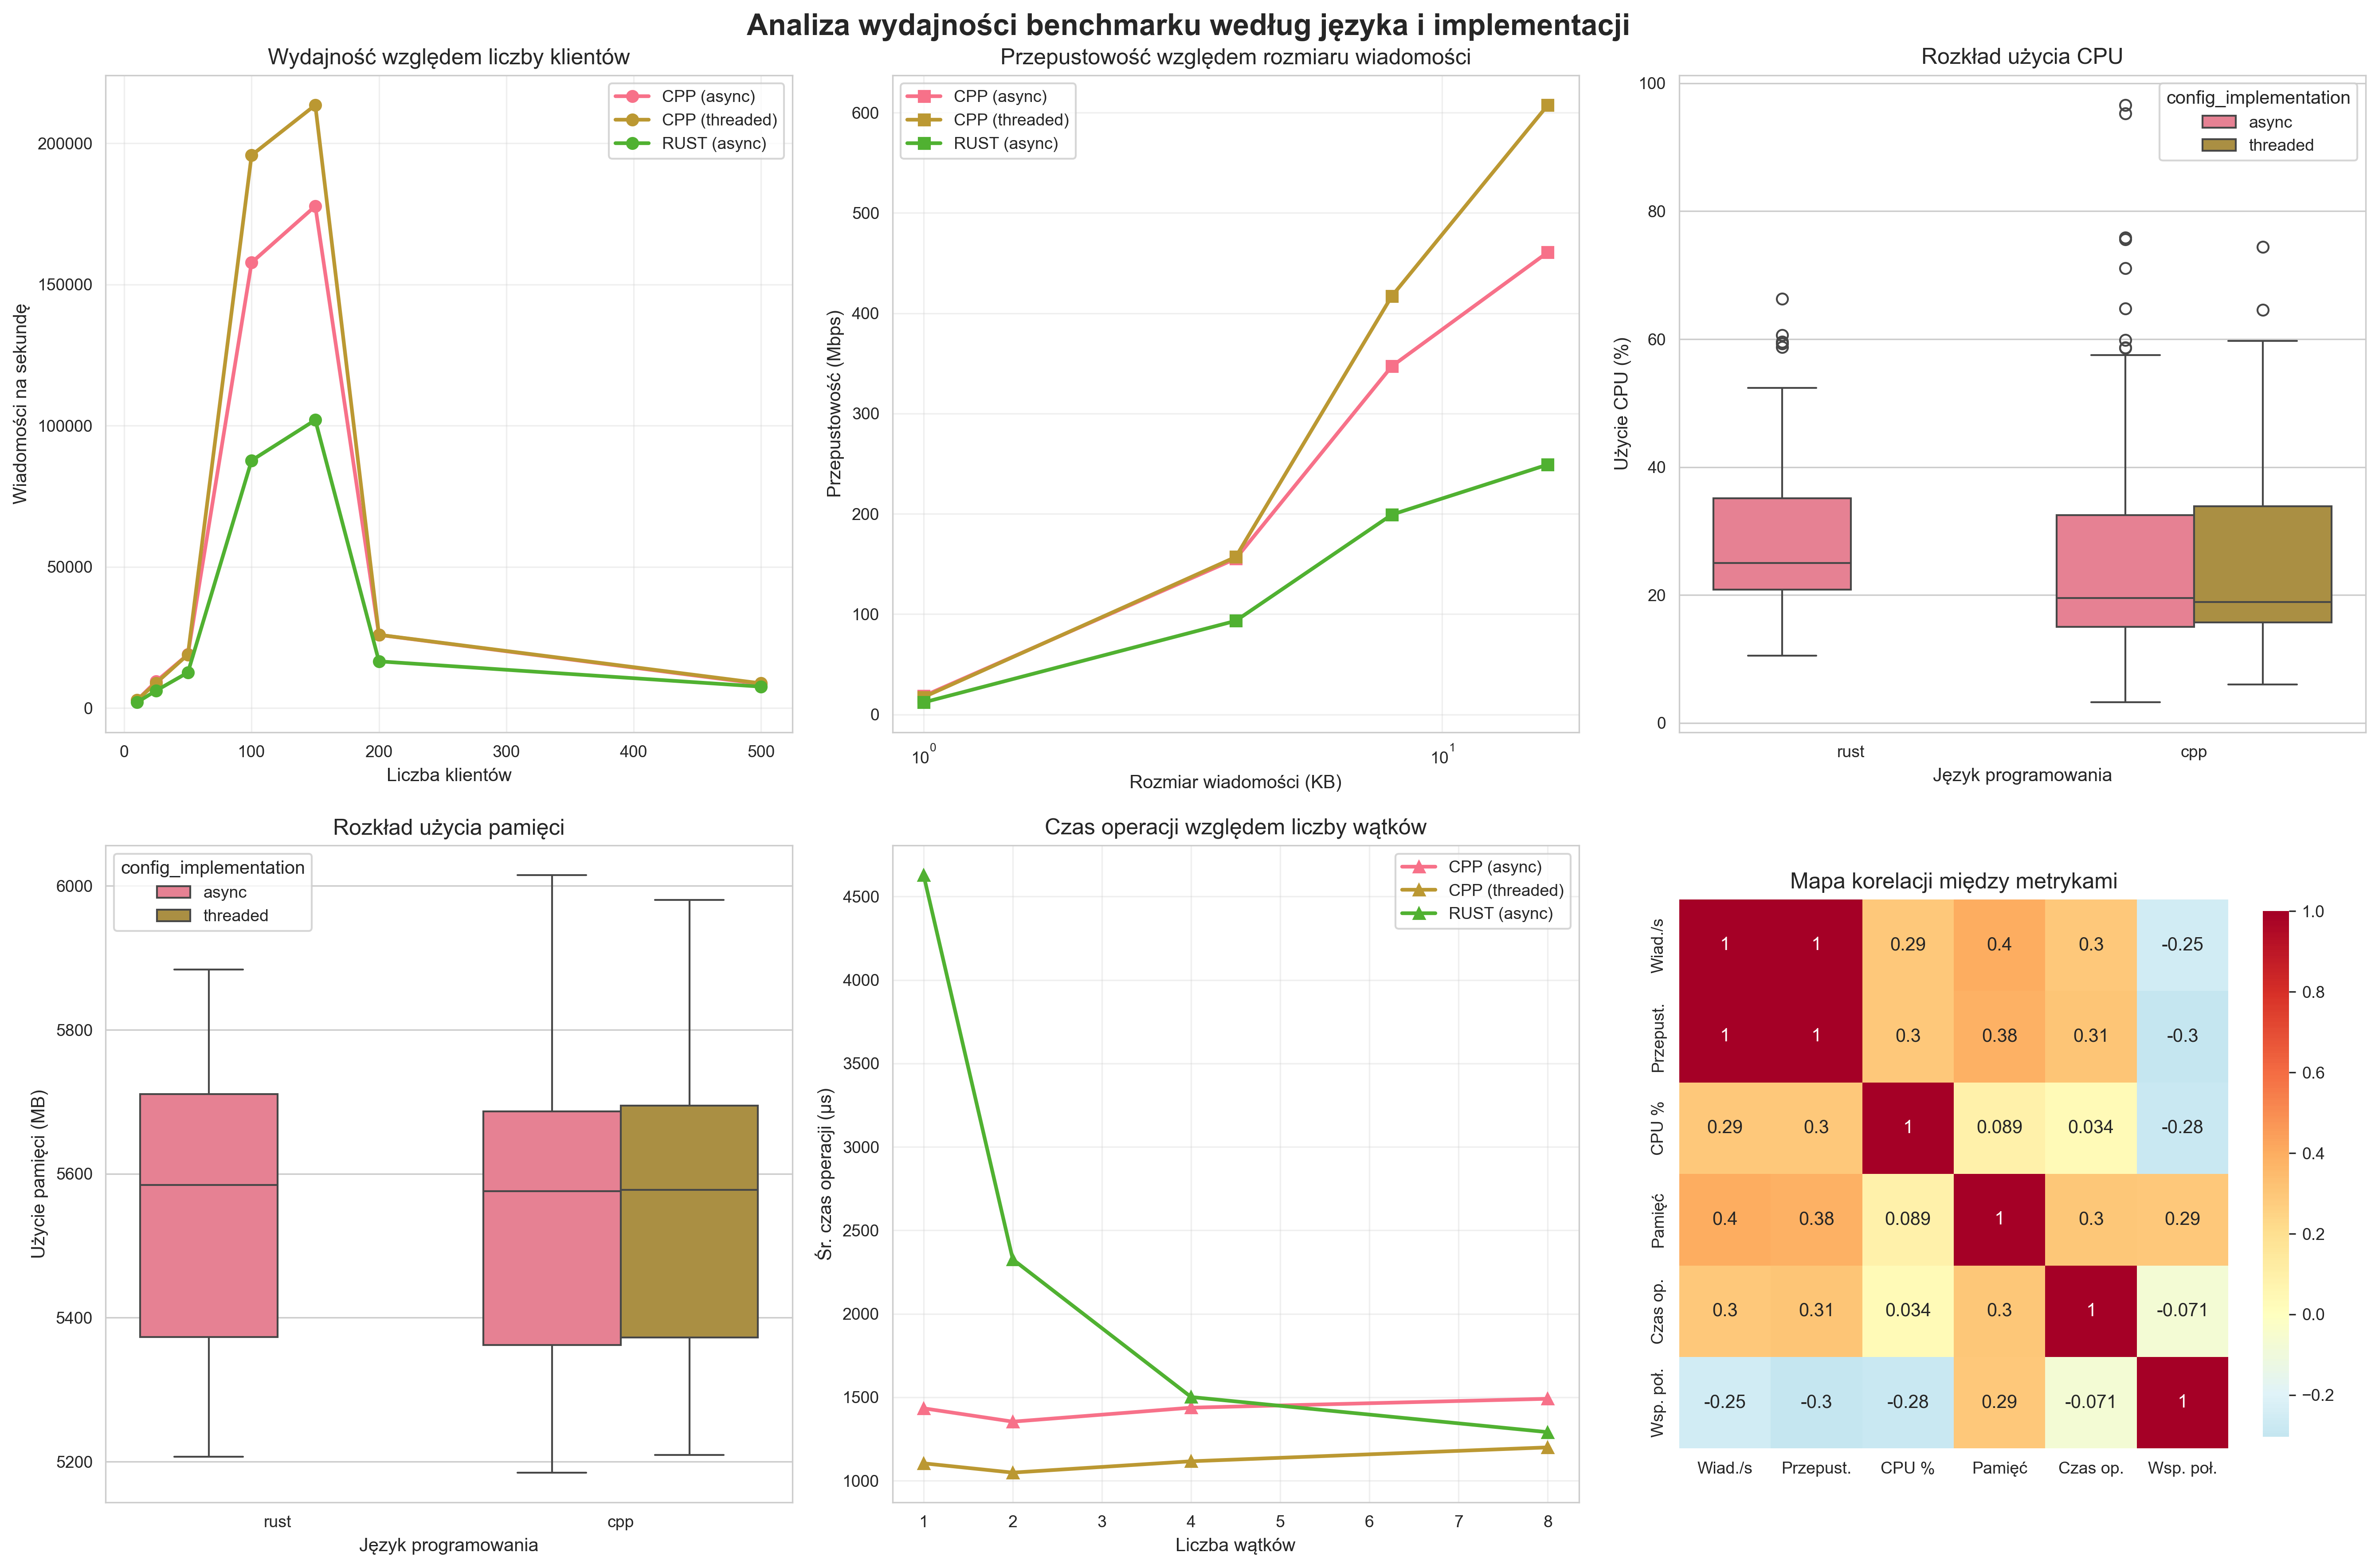
\includegraphics[width=0.9\textwidth]{analiza/images/conc/echo/arm/analiza_benchmarku.png}
    \caption{Analiza wyników benchmarku echo serwer}
    \label{analiza_benchmarku_echo_serwer}
\end{figure}
\subsubsection{Wydajność względem liczby klientów}
Przedstawiony w lewym górnym rogu wykres - rysunek \ref{analiza_benchmarku_echo_serwer} ilustruje zależność między liczbą obsługiwanych klientów a przepustowością (liczba wiadomości na sekundę) dla różnych implementacji serwera echo. Wykres uwidacznia charakterystyczne zachowanie systemów współbieżnych w warunkach rosnącego obciążenia. Implementacja w języku C++ w wariancie synchronicznym (threaded) osiąga najwyższą wydajność szczytową, około 210 000 wiadomości/s przy około 150 klientach, co znacząco przewyższa pozostałe implementacje. Implementacja asynchroniczna w C++ utrzymuje wydajność na poziomie około 180 000 wiadomości/s, natomiast implementacja Rust (asynchroniczna) osiąga maksymalną przepustowość na poziomie około 100 000 wiadomości/s.

Warto zauważyć charakterystyczny spadek wydajności wszystkich implementacji przy obciążeniu przekraczającym 150-200 klientów. Zjawisko to jest zgodne z teoretycznymi modelami systemów współbieżnych i wskazuje na osiągnięcie punktu nasycenia, gdzie koszty zarządzania kontekstem i synchronizacją zaczynają dominować nad rzeczywistą pracą użyteczną. Różnice między implementacjami mogą wynikać z odmiennych strategii zarządzania zasobami w obu językach oraz efektywności ich modeli współbieżności.

\subsubsection{Przepustowość względem rozmiaru wiadomości}
Centralny wykres górnego - rysunek \ref{analiza_benchmarku_echo_serwer} rzędu prezentuje przepustowość (wyrażoną w MB/s) w funkcji rozmiaru przetwarzanych wiadomości. Skala logarytmiczna na osi X pozwala na obserwację zachowania w szerokim zakresie wielkości komunikatów. Wszystkie badane implementacje wykazują wzrost przepustowości wraz ze zwiększaniem rozmiaru komunikatów, co jest oczekiwanym zjawiskiem wynikającym z redukcji względnych kosztów narzutu na operacje wejścia/wyjścia przy większych pakietach danych.

Implementacja synchroniczna w C++ osiąga najwyższą przepustowość, sięgającą 600 MB/s dla komunikatów o rozmiarze 10 KB. Implementacja asynchroniczna w C++ plasuje się na drugiej pozycji z wydajnością około 470 MB/s, podczas gdy implementacja Rust osiąga około \mbox{250 MB/s}. Warto zauważyć, że różnice wydajnościowe między implementacjami powiększają się wraz ze wzrostem rozmiaru komunikatów, co może sugerować odmienne optymalizacje mechanizmów buforowania i przetwarzania danych w badanych językach.

\subsubsection{Rozkład użycia CPU}
Wykres w prawym górnym rogu - rysunek \ref{analiza_benchmarku_echo_serwer} przedstawia rozkład procentowego wykorzystania procesora dla poszczególnych implementacji. Analiza wykresu pudełkowego wskazuje, że implementacja w języku Rust charakteryzuje się wyższą medianą wykorzystania CPU (około 28\%) w porównaniu z implementacją C++ (około 18-20\%). W przypadku języka C++ widoczne są pewne różnice między wariantami asynchronicznym i synchronicznym, przy czym wariant synchroniczny (threaded) wykazuje szerszą dystrybucję wartości, co może świadczyć o większej zmienności obciążenia procesora.

Występowanie wartości odstających, oznaczonych punktami powyżej górnych wąsów wykresu, wskazuje na sporadyczne skoki wykorzystania procesora, potencjalnie związane z operacjami zarządzania pamięcią, takimi jak mechanizm odśmiecania w przypadku Rusta lub zarządzanie pulami wątków w przypadku C++.

\subsubsection{Rozkład użycia pamięci}
Lewy dolny wykres - rysunek \ref{analiza_benchmarku_echo_serwer} prezentuje dystrybucję zużycia pamięci dla analizowanych implementacji. Mediany zużycia pamięci są zbliżone dla wszystkich implementacji i oscylują w~okolicach 5400-5500 MB. Implementacja w języku Rust charakteryzuje się nieznacznie wyższym medianym zużyciem pamięci, co może być związane z wewnętrznymi mechanizmami zarządzania własnością danych i zapewniania bezpieczeństwa pamięciowego.

Warto zauważyć, że implementacja synchroniczna w C++ wykazuje większy rozrzut wartości, co wskazuje na mniej przewidywalne charakterystyki alokacji pamięci. Może to być spowodowane dynamicznym tworzeniem i niszczeniem wątków, które generuje zmienne obciążenie mechanizmów zarządzania pamięcią. Implementacje asynchroniczne, zarówno w Rust, jak i C++, charakteryzują się bardziej stabilnym profilem pamięciowym, co jest typowe dla architektur opartych na pętlach zdarzeń.

\subsubsection{Czas operacji względem liczby wątków}
Środkowy dolny wykres - rysunek \ref{analiza_benchmarku_echo_serwer} ilustruje zależność między liczbą wątków a średnim czasem wykonania operacji (wyrażonym w mikrosekundach). Implementacja asynchroniczna w języku Rust wykazuje dramatyczny spadek czasu operacji przy zwiększeniu liczby wątków z \mbox{1 do 4}, co świadczy o efektywnym wykorzystaniu równoległości przez runtime Tokio. Po przekroczeniu 4 wątków zysk wydajnościowy maleje, co jest zgodne z prawem malejących zwrotów w kontekście przetwarzania równoległego.

Implementacje w języku C++ charakteryzują się bardziej stabilnymi czasami operacji w~funkcji liczby wątków, przy czym implementacja synchroniczna osiąga najniższe czasy, oscylujące wokół 1100 $\mu s$. Warto zauważyć, że przy większej liczbie wątków (6-8) różnice między implementacjami zmniejszają się, co sugeruje, że przy wystarczającej paralelizacji wydajność wszystkich podejść staje się ograniczona przez inne czynniki, takie jak opóźnienia sieci czy koszt przełączania kontekstu.

\subsubsection{Mapa korelacji między metrykami}
Prawy dolny wykres - rysunek \ref{analiza_benchmarku_echo_serwer} przedstawia macierz korelacji między różnymi metrykami wydajnościowymi. Wyraźnie widoczna jest silna dodatnia korelacja (wartość 1.0) między liczbą wiadomości na sekundę (Wiad/s) a przepustowością (Przepust.), co jest logiczną konsekwencją bezpośredniego związku tych metryk. Interesujące są umiarkowane korelacje między wykorzystaniem CPU a przepustowością (0.3) oraz pamięcią (0.089), co sugeruje, że zwiększone wykorzystanie zasobów procesora nie przekłada się liniowo na poprawę przepustowości.

Warto zwrócić uwagę na ujemne korelacje między czasem operacji (Czas op.) a przepustowością (-0.071) oraz między wskaźnikiem wydajności a zużyciem procesora (-0.28), co potwierdza intuicyjne oczekiwanie, że krótsze czasy operacji i mniejsze wykorzystanie zasobów przekładają się na wyższą wydajność systemu. Mapa korelacji dostarcza cennych informacji o współzależnościach między różnymi aspektami wydajności, co może być pomocne przy optymalizacji implementacji.

\subsubsection{Podsumowanie}
Przeprowadzona analiza porównawcza implementacji serwerów echo w językach Rust i C++ wskazuje na znaczące różnice w charakterystykach wydajnościowych różnych podejść do przetwarzania współbieżnego. Implementacja synchroniczna w C++ osiąga najwyższą przepustowość w warunkach optymalnego obciążenia, jednak cechuje się większą zmiennością zużycia zasobów. Implementacja asynchroniczna w C++ oferuje kompromis między wydajnością a stabilnością, podczas gdy implementacja asynchroniczna w języku Rust, choć charakteryzuje się niższą bezwzględną przepustowością, wykazuje najbardziej efektywne skalowanie w funkcji liczby wątków.

Wyniki badań sugerują, że wybór optymalnego modelu programowania współbieżnego powinien uwzględniać nie tylko surowe metryki wydajnościowe, ale również charakterystyki stabilności, przewidywalności i efektywności skalowania. W rzeczywistych zastosowaniach sieciowych, gdzie kluczowe znaczenie ma niezawodność i przewidywalność działania systemu, podejście asynchroniczne, szczególnie zaimplementowane w języku Rust, może oferować korzystniejsze kompromisy między wydajnością a stabilnością i bezpieczeństwem niż tradycyjne podejście oparte na puli wątków.

\subsection{Wyniki benchmarków - platforma x86\_64}
\begin{figure}[H]
    \centering
    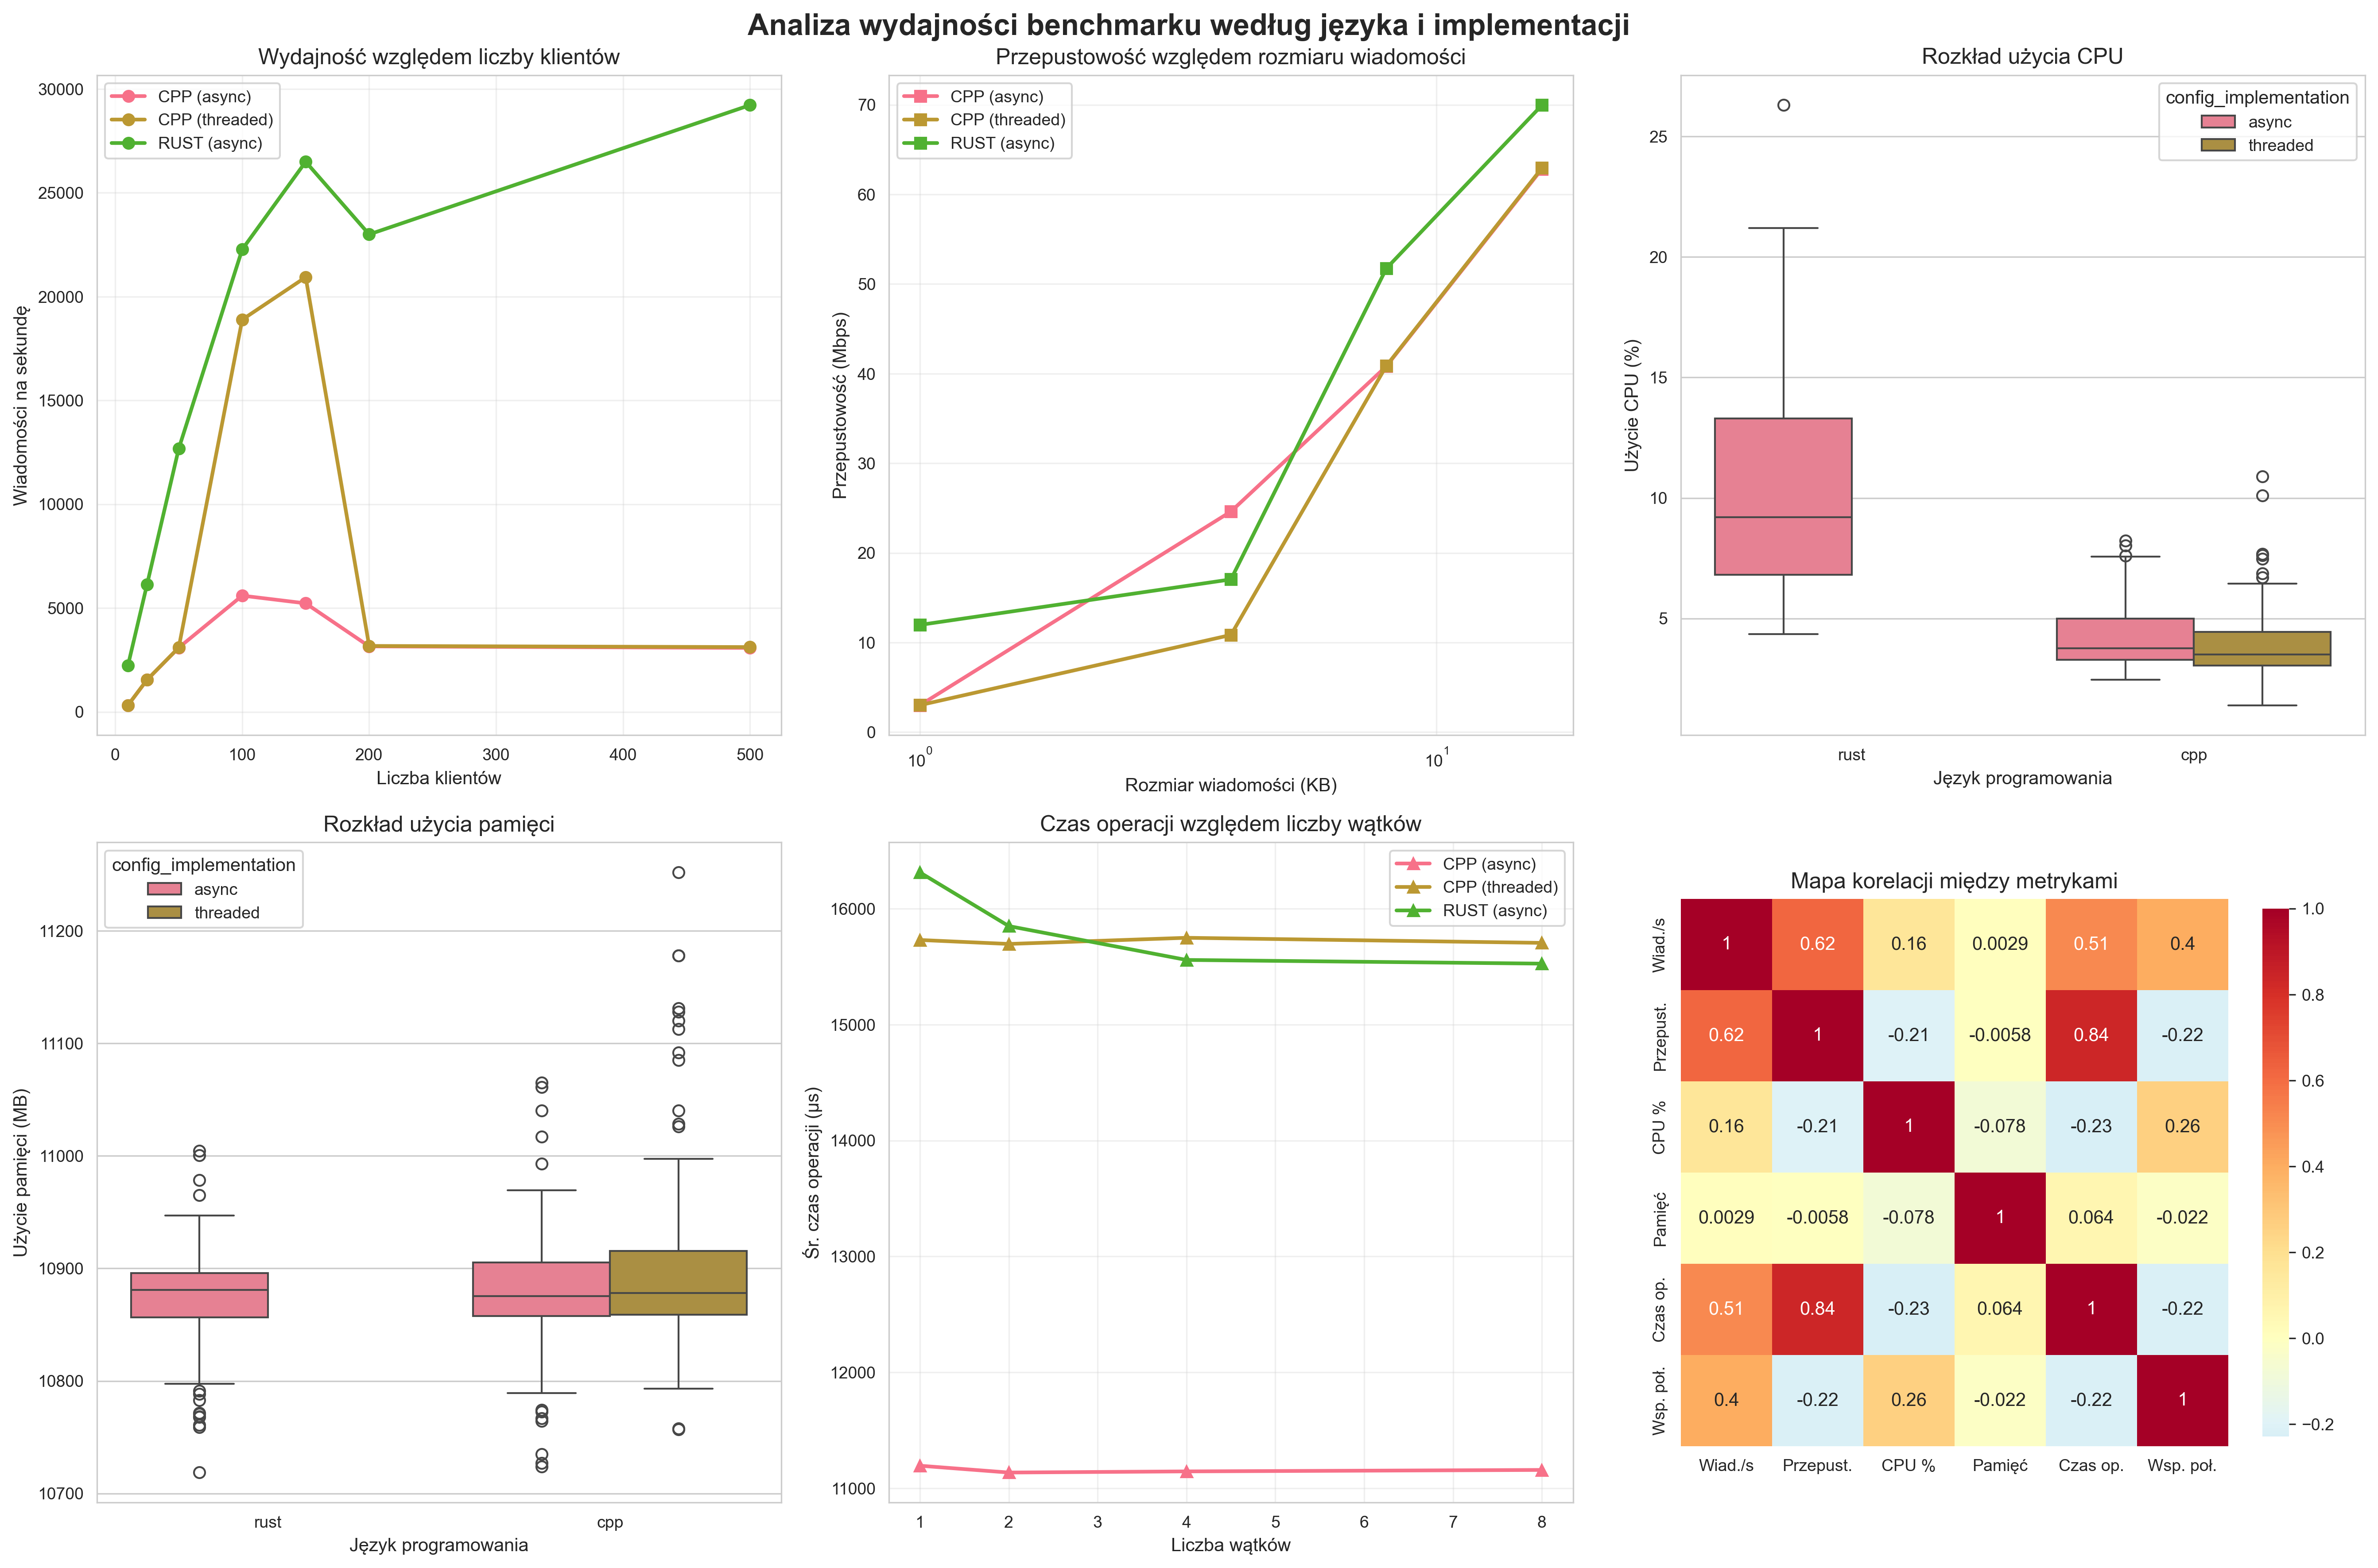
\includegraphics[width=0.9\textwidth]{analiza/images/conc/echo/x86/analiza_benchmarku.png}
    \caption{Analiza wyników benchmarku echo serwer}
    \label{analiza_benchmarku_echo_serwer_x86_64}
\end{figure}

\subsubsection{Wydajność względem liczby klientów}
Pierwszy wykres (lewy górny) - rysunek \ref{analiza_benchmarku_echo_serwer_x86_64} przedstawia zależność między liczbą jednoczesnych klientów a przepustowością mierzoną liczbą przetwarzanych wiadomości na sekundę. Implementacja asynchroniczna w języku Rust (oznaczona kolorem zielonym) wykazuje znacząco wyższą wydajność w porównaniu do obu implementacji w języku C++. Przepustowość implementacji w Rust wzrasta niemal liniowo wraz ze zwiększaniem liczby klientów, osiągając szczyt około 26 000 wiadomości/s przy 150 klientach, po czym następuje niewielki spadek i~ponowny wzrost do prawie 30 000 wiadomości/s przy 500 klientach.

W przypadku implementacji opartej na wątkach w C++ (oznaczona kolorem żółtym) obserwujemy początkowy wzrost wydajności do około 21 000 wiadomości/s przy 150 klientach, po którym następuje gwałtowny spadek do około 3 000 wiadomości/s dla większej liczby klientów. Implementacja asynchroniczna w C++ (kolor różowy) wykazuje najniższą wydajność spośród badanych rozwiązań, osiągając maksymalnie około 5 500 wiadomości/s.

\subsubsection{ Przepustowość względem rozmiaru wiadomości}
Środkowy wykres górny - rysunek \ref{analiza_benchmarku_echo_serwer_x86_64} ilustruje zależność przepustowości (wyrażonej w MB/s) od rozmiaru przesyłanych wiadomości w skali logarytmicznej. Wszystkie implementacje wykazują wzrost przepustowości wraz ze zwiększaniem rozmiaru komunikatów, co jest zgodne z~teoretycznymi założeniami dotyczącymi amortyzacji kosztów stałych operacji wejścia/wyjścia.

Implementacja asynchroniczna w języku Rust (kolor zielony) osiąga najwyższą przepustowość, sięgającą 70 MB/s dla komunikatów o rozmiarze 10 KB. Implementacja wykorzystująca wątki w C++ (kolor żółty) osiąga około 63 MB/s, natomiast implementacja asynchroniczna w~C++ (kolor różowy) wykazuje najniższą wydajność w zakresie większych komunikatów, choć warto zauważyć jej relatywnie dobrą wydajność dla małych wiadomości (około 1 KB).

\subsubsection{Rozkład użycia CPU}
Prawy górny wykres - rysunek \ref{analiza_benchmarku_echo_serwer_x86_64} prezentuje rozkład procentowego użycia procesora (CPU) przez poszczególne implementacje. Implementacja w języku Rust (kolor czerwony) charakteryzuje się zdecydowanie wyższym zużyciem zasobów procesora, z medianą na poziomie około 9-10\% i górnym kwartylem sięgającym 13\%. Implementacje w C++ wykazują znacząco niższe zużycie CPU, z medianami na poziomie 4-5\%. Warto zauważyć pojedyncze wartości odstające w przypadku implementacji Rust, sięgające nawet 26\% wykorzystania procesora.

Mniejsze zużycie CPU przez implementacje C++ może sugerować bardziej efektywne wykorzystanie zasobów procesorowych, jednak w połączeniu z niższą wydajnością (zwłaszcza w~przypadku implementacji asynchronicznej) może również wskazywać na niepełne wykorzystanie dostępnej mocy obliczeniowej.

\subsubsection{Rozkład użycia pamięci}
Lewy dolny wykres - rysunek \ref{analiza_benchmarku_echo_serwer_x86_64} przedstawia dystrybucję zużycia pamięci (w MB) dla badanych implementacji. Wszystkie rozwiązania charakteryzują się zbliżonym medianym poziomem zużycia pamięci, oscylującym wokół 10 900 MB. Implementacja wykorzystująca wątki w C++ (kolor brązowy) wykazuje nieznacznie wyższe zużycie pamięci oraz większy rozrzut wartości, co może być związane z dodatkową pamięcią wymaganą do zarządzania kontekstem wątków.

Obecność wartości odstających (szczególnie w przypadku implementacji w C++) sugeruje sporadyczne zwiększone zapotrzebowanie na pamięć, potencjalnie związane z operacjami buforowania lub nagłymi wzrostami obciążenia. Ogólnie niewielkie różnice w zużyciu pamięci między implementacjami wskazują, że aspekt pamięciowy nie stanowi kluczowego czynnika różnicującego wydajność badanych rozwiązań.

\subsubsection{Czas operacji względem liczby wątków}
Środkowy dolny wykres - rysunek \ref{analiza_benchmarku_echo_serwer_x86_64} prezentuje zależność średniego czasu operacji (w mikrosekundach) od liczby wykorzystywanych wątków. Implementacja asynchroniczna w języku Rust (kolor zielony) wykazuje najwyższy początkowy czas operacji (około 16 500 $\mu s$ przy jednym wątku), który ulega poprawie wraz ze zwiększaniem liczby wątków, osiągając poziom zbliżony do implementacji opartej na wątkach w C++ przy 8 wątkach.

Implementacja wykorzystująca wątki w C++ (kolor żółty) utrzymuje względnie stały czas operacji na poziomie około 15 700 $
mu s$ niezależnie od liczby wątków, co sugeruje niewielką korzyść z dodatkowej paralelizacji. Implementacja asynchroniczna w C++ (kolor różowy) charakteryzuje się najniższymi czasami operacji (około 11 100 $\mu s$) i wykazuje najmniejszą zmienność w funkcji liczby wątków.

\subsubsection{Mapa korelacji między metrykami}
Prawy dolny wykres -rysunek \ref{analiza_benchmarku_echo_serwer_x86_64} przedstawia macierz korelacji między różnymi metrykami wydajnościowymi. Szczególnie istotna jest silna dodatnia korelacja (0,84) między przepustowością a czasem operacji, co może wskazywać, że dłuższy czas przetwarzania pojedynczej operacji przekłada się na wyższą przepustowość całego systemu przy odpowiednim poziomie równoległości.

Umiarkowana dodatnia korelacja (0,62) między liczbą wiadomości na sekundę a przepustowością potwierdza oczekiwaną zależność między tymi powiązanymi metrykami. Interesujące są również negatywne korelacje między procentowym wykorzystaniem CPU a przepustowością \mbox{(-0,21)} oraz między wskaźnikiem wydajności a zużyciem pamięci (-0,078), sugerujące, że wyższe obciążenie zasobów nie przekłada się bezpośrednio na lepszą wydajność.

\subsubsection{Podsumowanie}
Wyniki sugerują, że asynchroniczny model programowania w języku Rust, wykorzystujący zaawansowany system zarządzania zadaniami, oferuje najkorzystniejszy kompromis między wydajnością a skalowalnością dla wymagających zastosowań sieciowych. Implementacja wykorzystująca wielowątkowość w C++ może stanowić rozsądną alternatywę dla systemów o~umiarkowanym obciążeniu, podczas gdy model asynchroniczny w C++ może być preferowany w sytuacjach, gdzie krytyczne znaczenie ma minimalizacja opóźnień pojedynczych operacji.

\subsection{Porównanie pomiędzy platformami}
\begin{figure}[H]
    \centering
    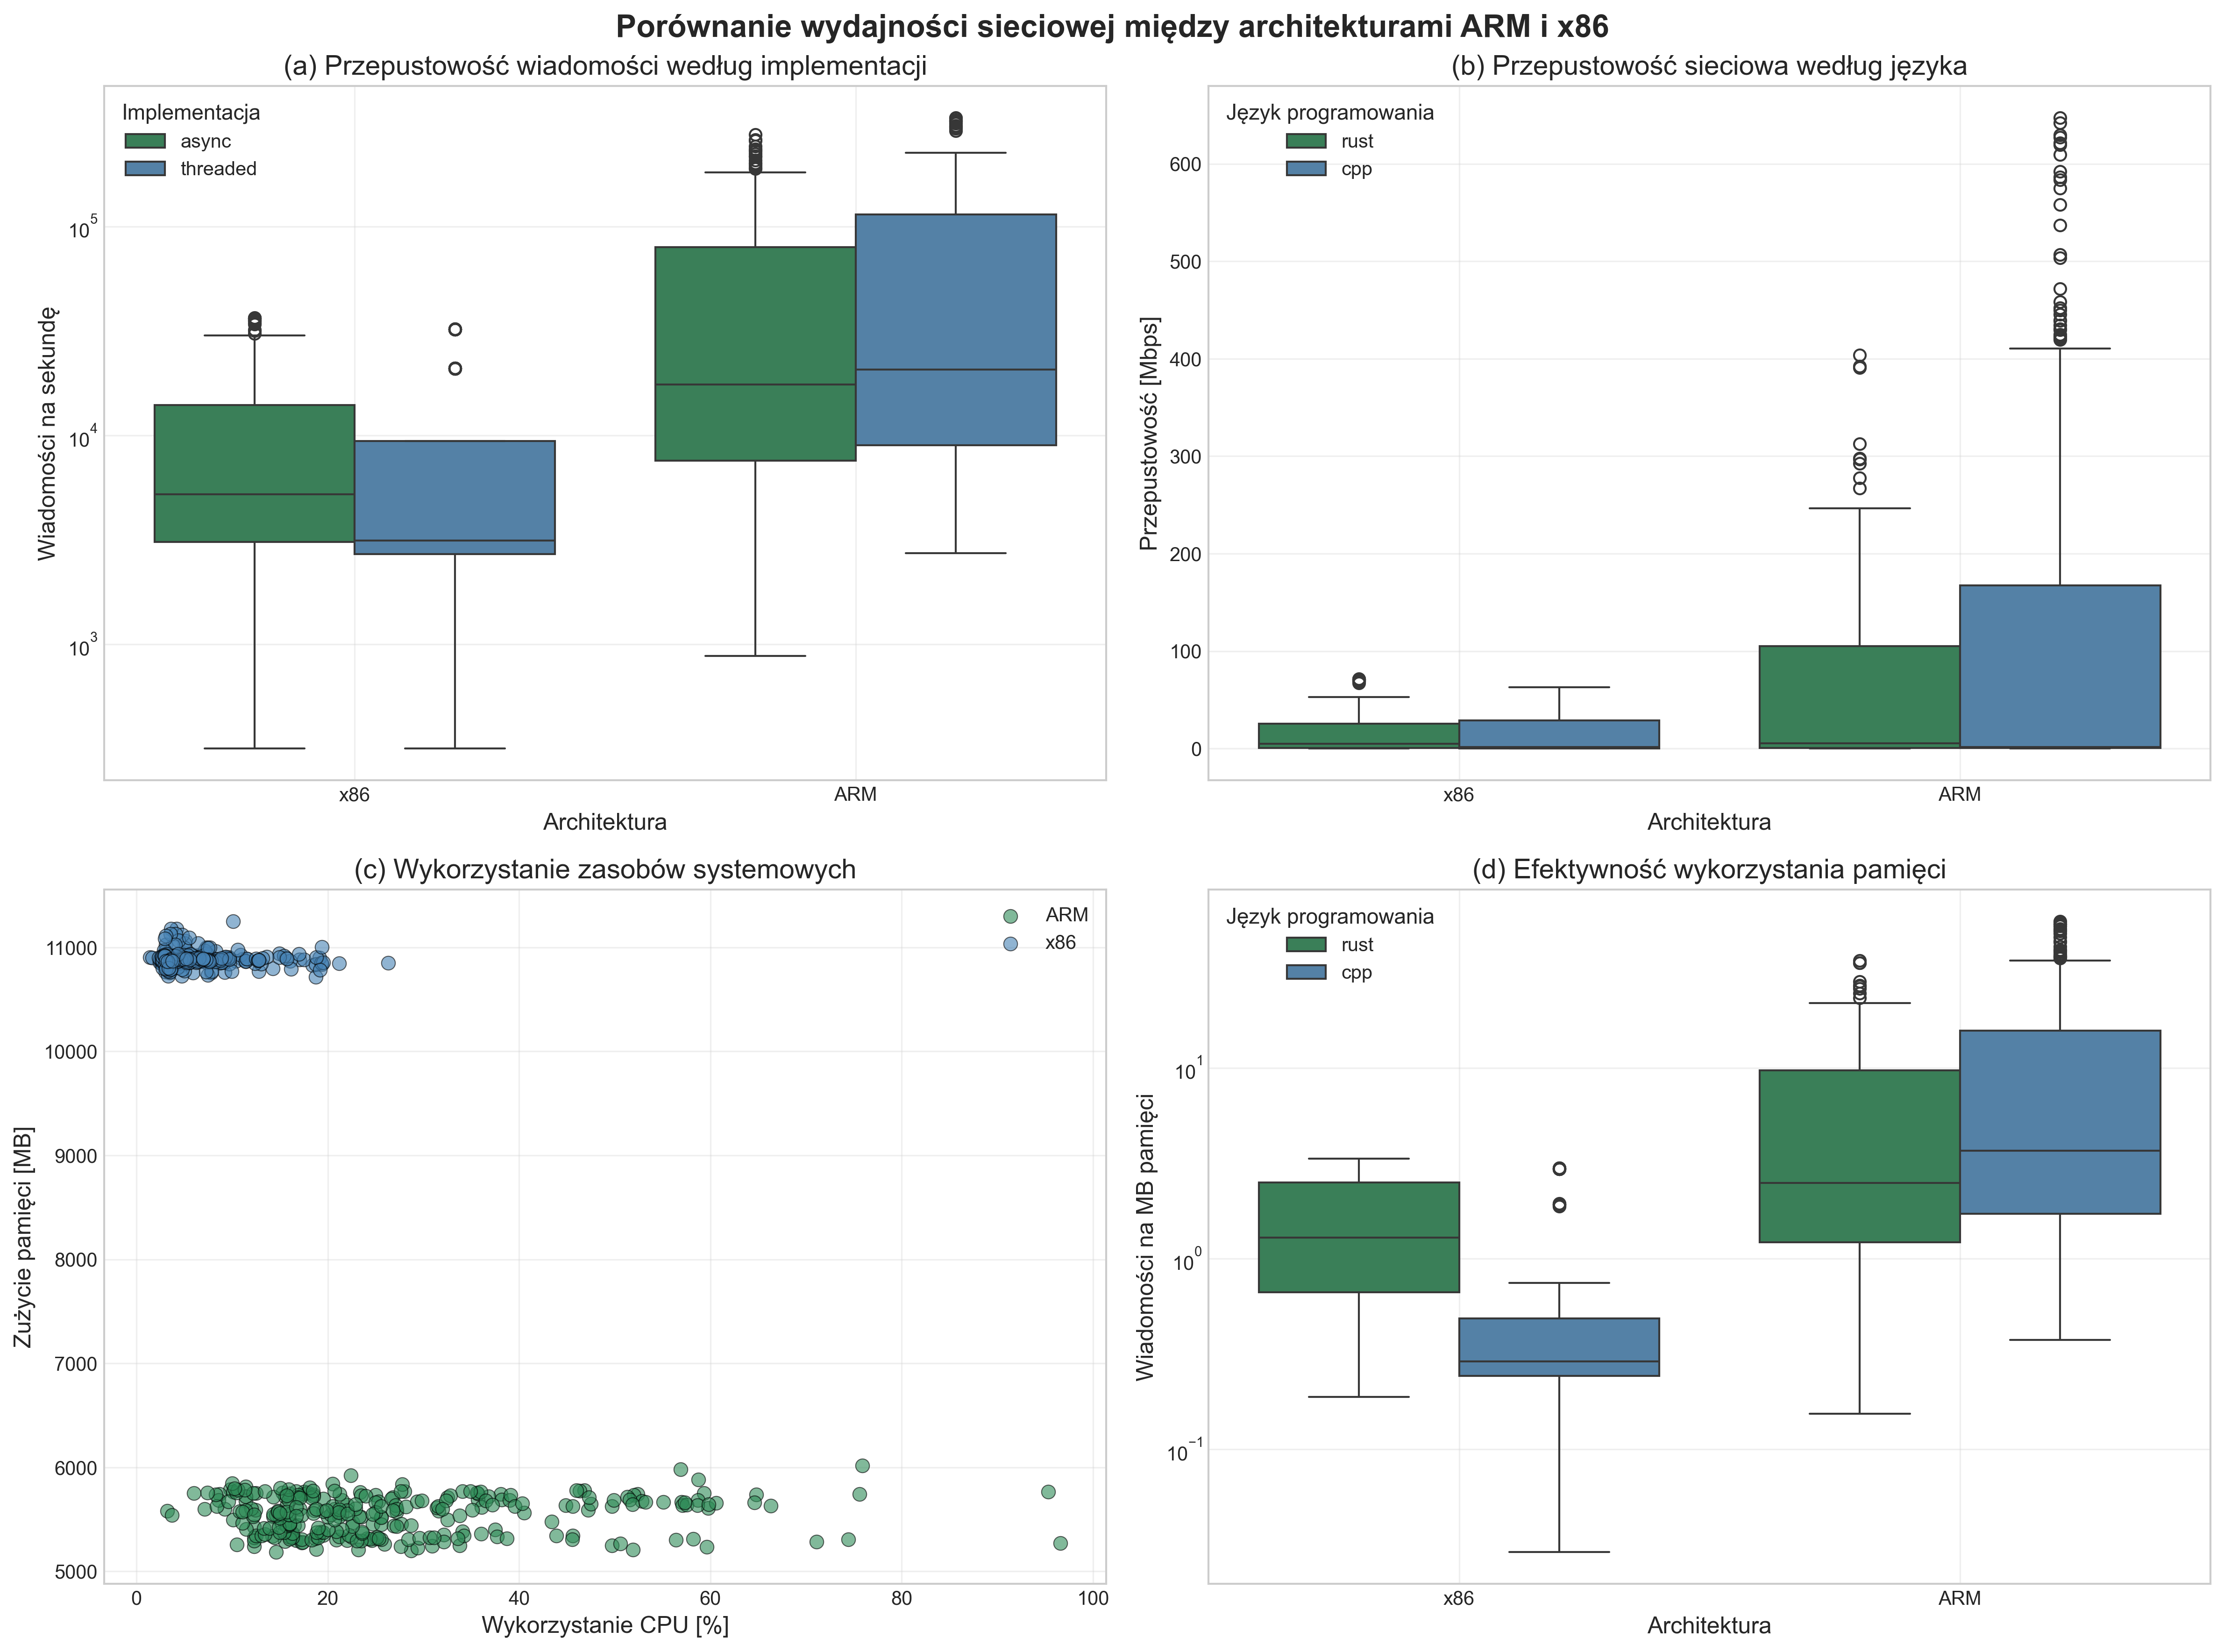
\includegraphics[width=0.9\textwidth]{analiza/images/conc/echo/compare/rysunek_1_wydajnosc_sieciowa.png}
    \caption{Porównanie wydajności sieciowej pomiędzy platformami ARM i x86\_64}
    \label{rysunek_1_wydajnosc_sieciowa}
\end{figure}
\subsubsection{Przepustowość wiadomości według implementacji}
Wykres (a) - rysunek \ref{rysunek_1_wydajnosc_sieciowa} przedstawia porównanie przepustowości komunikacji sieciowej, wyrażonej liczbą wiadomości na sekundę, dla architektur x86 i ARM, z uwzględnieniem dwóch typów implementacji: asynchronicznej (kolor zielony) i wątkowej (kolor niebieski). Analiza wykresu wskazuje na dramatyczną różnicę wydajnościową na korzyść architektury ARM:
\begin{itemize}
    \item Implementacje na architekturze x86 osiągają przepustowość rzędu $10^1$-$10^2$ wiadomości/s, z medianą około 5-10 wiadomości/s niezależnie od typu implementacji.
    \item Implementacje na architekturze ARM wykazują przepustowość o 1-2 rzędy wielkości wyższą, osiągając $10^3$-$10^5$ wiadomości/s, z~medianą około $3$-$4\times10^4$ wiadomości/s.
    \item Implementacja wątkowa na ARM osiąga nieznacznie wyższą wydajność median niż implementacja asynchroniczna, podczas gdy na x86 różnica między typami implementacji jest marginalna.
\end{itemize}

\subsubsection{Przepustowość sieciowa według języka programowania}
Wykres (b) - rysunek \ref{rysunek_1_wydajnosc_sieciowa} ilustruje przepustowość sieciową wyrażoną w megabitach na sekundę (Mbps), z podziałem na architektury i języki programowania: Rust (kolor zielony) i C++ (kolor niebieski). Obserwujemy:
\begin{itemize}
    \item Architektura ARM osiąga średnią przepustowość około 100 Mbps, podczas gdy x86 jedynie około 20-30 Mbps.
    \item Implementacje w języku C++ na ARM wykazują nieznacznie wyższą medianę przepustowości niż implementacje w Rust, osiągając około 170 Mbps wobec 100 Mbps.
    \item Charakterystyczna jest obecność licznych wartości odstających dla implementacji ARM, z~niektórymi punktami przekraczającymi 600 Mbps, co wskazuje na potencjał do osiągania szczytowej wydajności w optymalnych warunkach.
\end{itemize}


\subsubsection{Wykorzystanie zasobów systemowych}
Wykres (c) - rysunek \ref{rysunek_1_wydajnosc_sieciowa} przedstawia zależność między zużyciem pamięci (oś y, w MB) a wykorzystaniem procesora (oś x, w procentach) dla obu architektur: ARM (punkty zielone) i x86 (punkty niebieskie). Analiza tego wykresu ujawnia fundamentalne różnice w profilu wykorzystania zasobów:
\begin{itemize}
    \item Implementacje na architekturze x86 charakteryzują się zużyciem pamięci na poziomie około 11 000 MB (11 GB), co jest wartością niemal dwukrotnie wyższą niż w przypadku ARM.
    \item Implementacje ARM wykazują zużycie pamięci w zakresie 5 500-6 000 MB (5,5-6 GB).
    \item Wykorzystanie procesora jest bardziej zróżnicowane, ale generalnie podobne dla obu architektur, z punktami dla ARM rozproszonymi od niemal 0\% do blisko 100\% CPU, przy czym większość obserwacji koncentruje się poniżej 60\%.
    \item Dla architektury x86 większość punktów grupuje się w przedziale 0-30\% wykorzystania CPU.
\end{itemize}

\subsubsection{Efektywność wykorzystania pamięci}
Wykres (d) - rysunek \ref{rysunek_1_wydajnosc_sieciowa} prezentuje efektywność wykorzystania pamięci, wyrażoną liczbą przetworzonych wiadomości na megabajt (wiadomości/MB), z podziałem na architektury i języki programowania. Obserwacje:
\begin{itemize}
    \item Architektura ARM charakteryzuje się znacząco wyższą efektywnością pamięciową niż x86, osiągając medianę około 3-5 wiadomości/MB, podczas gdy x86 osiąga jedynie 0,3-1 wiadomości/MB.
    \item Na architekturze x86 implementacje w Rust (zielony) wykazują wyższą efektywność pamięciową niż implementacje C++ (niebieski), z medianą około 1 wiadomości/MB wobec \mbox{0,3 wiadomości/MB}.
    \item Na architekturze ARM różnica między językami jest mniej wyraźna, choć C++ nadal wykazuje nieznacznie niższą efektywność pamięciową.
    \item Skala logarytmiczna na osi pionowej podkreśla istotne różnice rzędu wielkości w efektywności między architekturami.
\end{itemize}

\subsubsection{Podsumowanie}
Przeprowadzona analiza porównawcza wydajności sieciowej między architekturami ARM i x86 ujawnia wyraźną przewagę architektury ARM w niemal wszystkich badanych aspektach. ARM oferuje znacząco wyższą przepustowość komunikacji, zarówno w liczbie wiadomości na sekundę, jak i w megabitach na sekundę, przy jednoczesnym zużyciu tylko około połowy pamięci wymaganej przez implementacje x86. Ponadto, efektywność wykorzystania pamięci jest o rząd wielkości wyższa na architekturze ARM.

\begin{figure}[H]
    \centering
    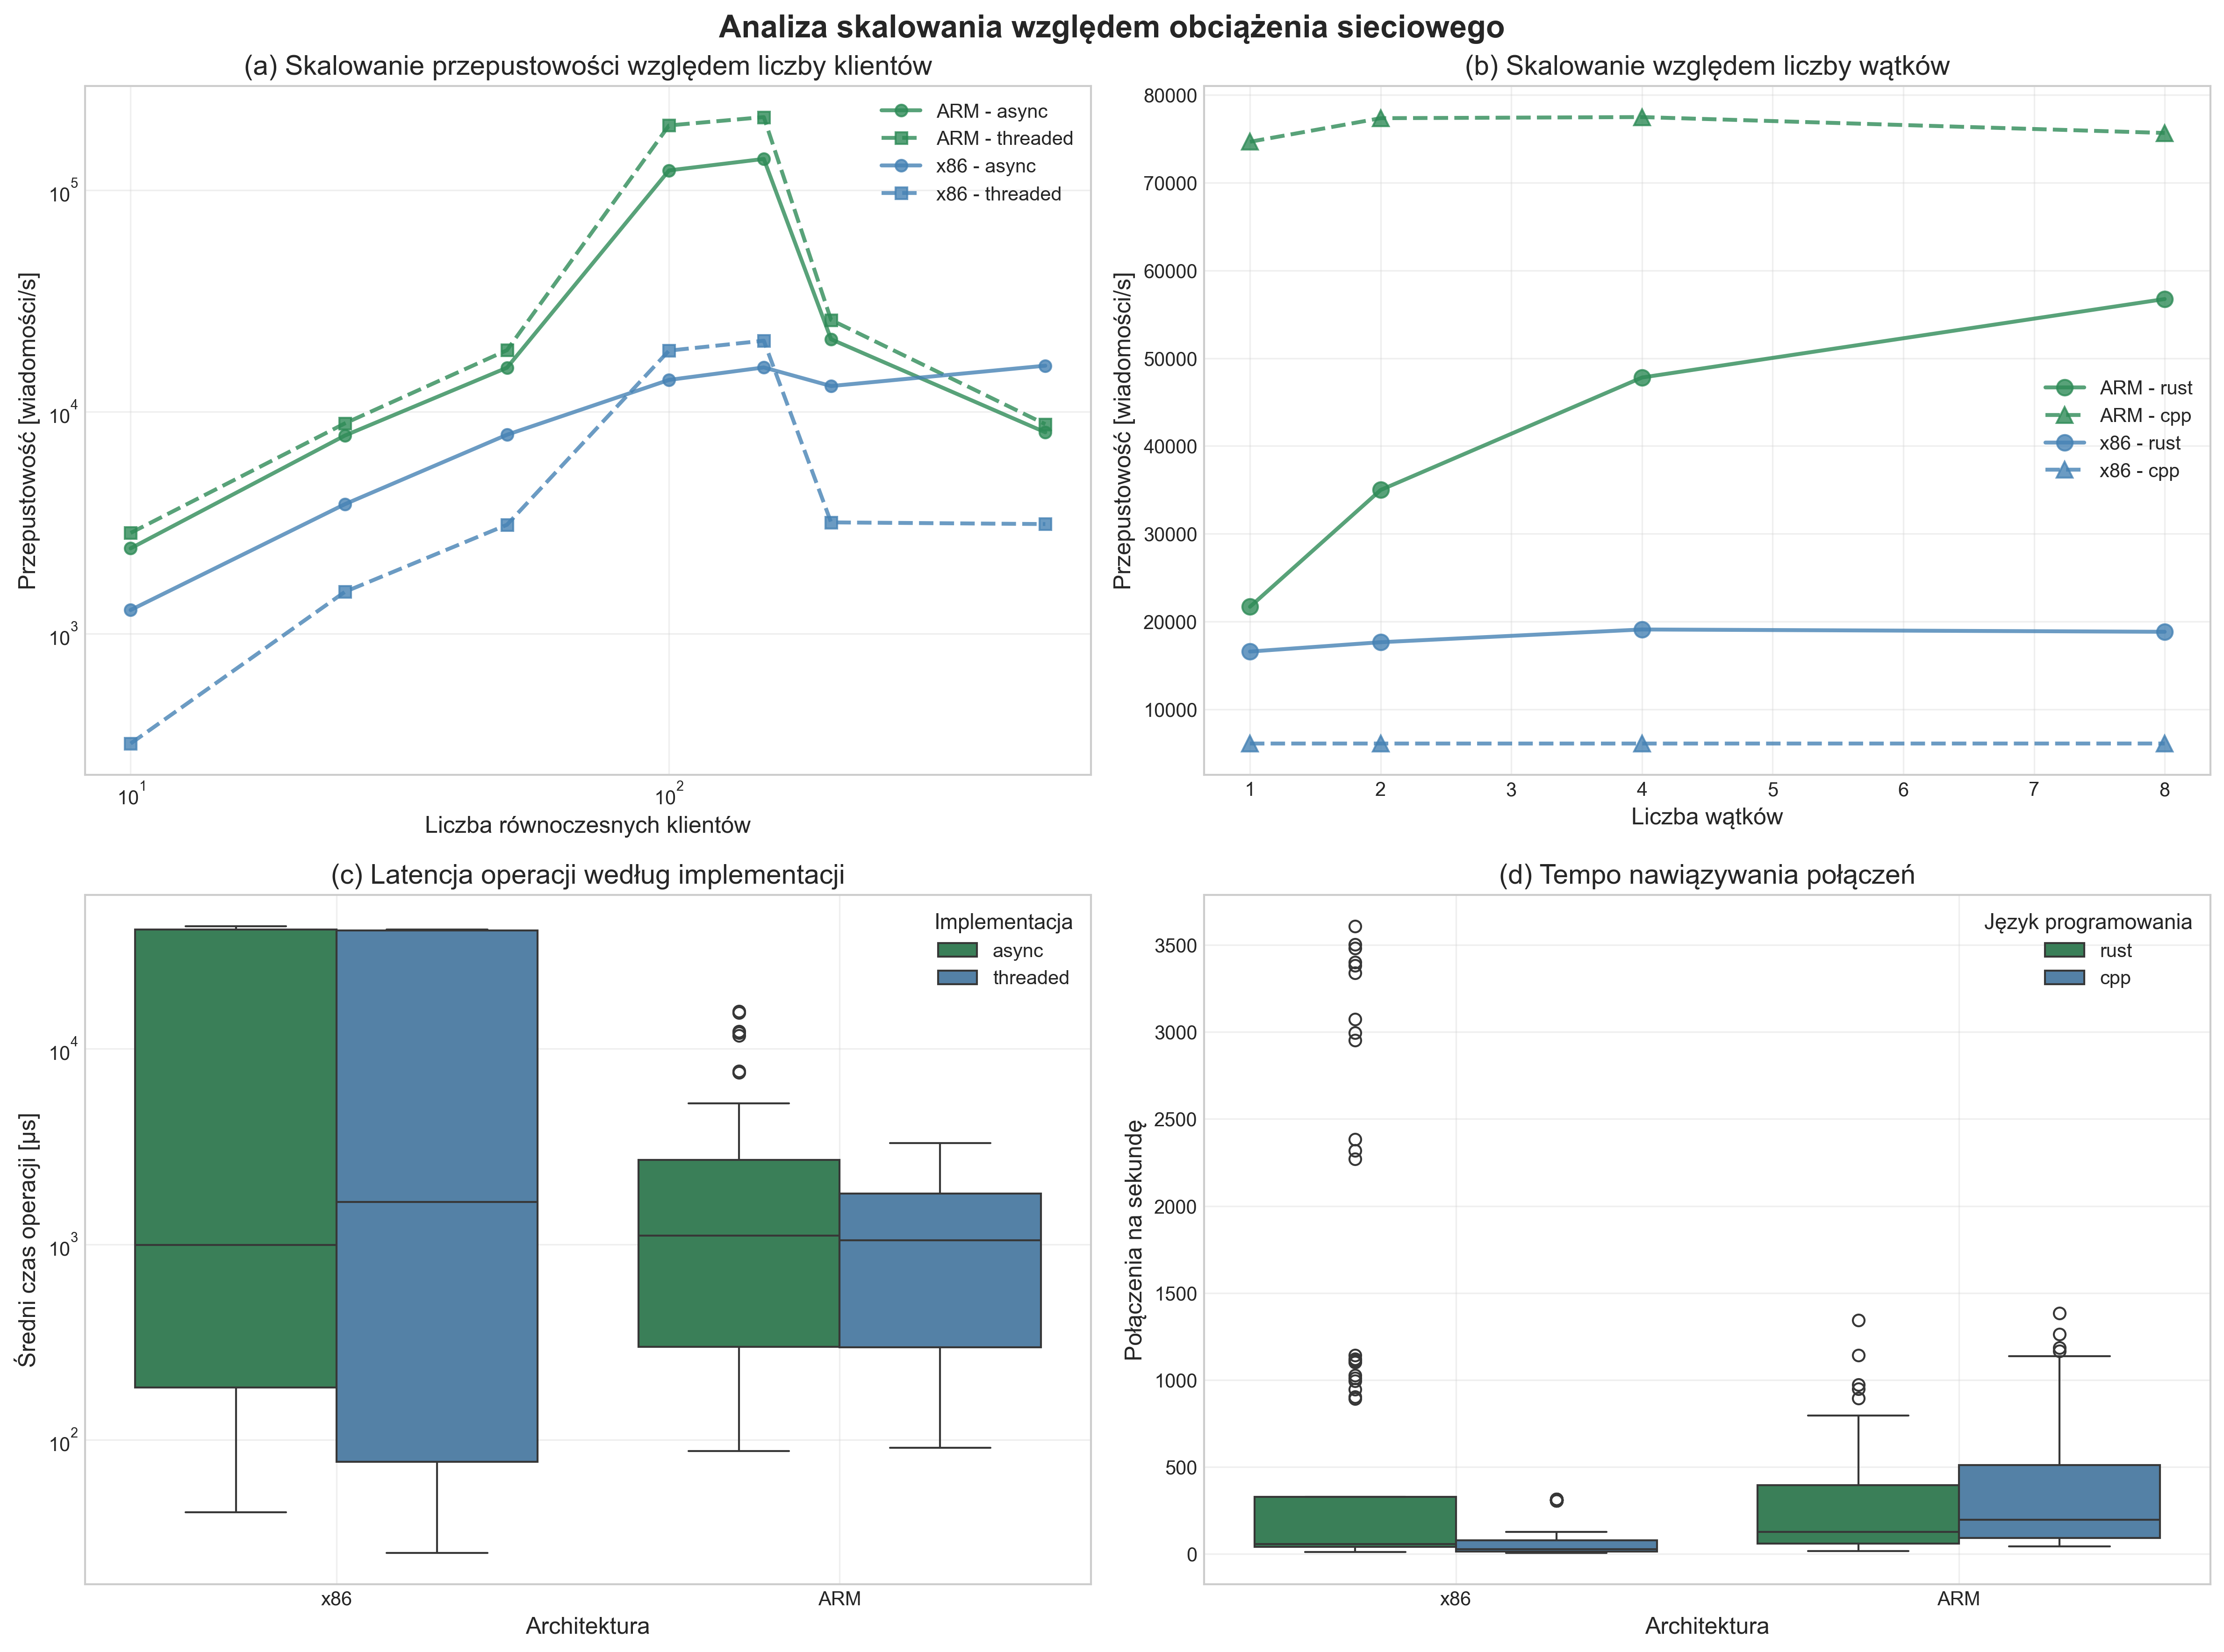
\includegraphics[width=0.9\textwidth]{analiza/images/conc/echo/compare/rysunek_2_skalowanie_obciazenia.png}
    \caption{Analiza skalowania względem obciążenia sieciowego}
    \label{rysunek_2_skalowanie_obciazenia}
\end{figure}
\subsubsection{Skalowanie przepustowości względem liczby klientów}
Wykres (a) - rysunek \ref{rysunek_2_skalowanie_obciazenia} przedstawia zależność przepustowości komunikacji sieciowej od liczby równoczesnych klientów dla dwóch architektur (ARM i x86) oraz dwóch metod implementacji (asynchronicznej i wątkowej). Analiza ujawnia znaczące różnice w charakterystyce skalowania:
\begin{itemize}
    \item Implementacje na architekturze ARM (linie zielone) osiągają przepustowość o rząd wielkości wyższą niż implementacje na x86 (linie niebieskie), szczególnie w obszarze optymalnego obciążenia (około 100 klientów).
    \item Obie architektury wykazują charakterystyczną krzywą skalowania w kształcie dzwonu, osiągając szczyt wydajności przy około 100 równoczesnych klientach, po czym następuje spadek przepustowości wraz z dalszym wzrostem liczby klientów.
    \item Implementacja wątkowa na ARM (zielona linia przerywana) osiąga najwyższą przepustowość, sięgającą ponad $10^5$ wiadomości na sekundę w punkcie szczytowym, podczas gdy analogiczna implementacja na x86 osiąga około $2\times10^4$ wiadomości na sekundę.
    \item Godny uwagi jest fakt, że implementacja wątkowa na x86 (niebieska linia przerywana) wykazuje najniższą początkową wydajność przy małej liczbie klientów, ale jednocześnie najszybsze tempo wzrostu przepustowości w zakresie 10-100 klientów.
\end{itemize}


\subsubsection{Skalowanie względem liczby wątków}
Wykres (b) - rysunek \ref{rysunek_2_skalowanie_obciazenia} ilustruje zależność przepustowości od liczby wątków roboczych dla dwóch architektur i dwóch języków programowania (Rust i C++). Obserwacje:
\begin{itemize}
    \item Implementacja C++ na architekturze ARM (zielone trójkąty, linia przerywana) wykazuje najwyższą przepustowość, utrzymującą się na stabilnym poziomie około 75 000 wiadomości na sekundę niezależnie od liczby wątków.
    \item Implementacja Rust na ARM (zielone kółka, linia ciągła) demonstruje doskonałą skalowalność, zwiększając przepustowość z około 20 000 do 55 000 wiadomości/s przy zwiększeniu liczby wątków z 1 do 8.
    \item Implementacja Rust na x86 (niebieskie kółka, linia ciągła) wykazuje minimalne korzyści ze zwiększania liczby wątków, utrzymując przepustowość na poziomie 15 000-20 000 wiadomości/s.
    \item Implementacja C++ na x86 (niebieskie trójkąty, linia przerywana) osiąga najniższą wydajność, utrzymując się na stałym poziomie około 5 000-6 000 wiadomości/s niezależnie od liczby wątków.
\end{itemize}

\subsubsection{Latencja operacji według implementacji}
Wykres (c) - rysunek \ref{rysunek_2_skalowanie_obciazenia} przedstawia rozkład czasów opóźnienia operacji sieciowych (latencji) w mikrosekundach ($\mu s$) dla różnych implementacji i architektur:
\begin{itemize}
    \item Architektura ARM charakteryzuje się ogólnie niższą medianą latencji (około 500-600 $\mu s$) w~porównaniu do x86 (około 1 000 $\mu s$).
    \item Implementacje na architekturze x86 wykazują znacznie większy rozrzut wartości latencji, co wskazuje na mniej przewidywalne czasy odpowiedzi, szczególnie dla implementacji asynchronicznej (zielony wykres pudełkowy).
    \item Implementacja wątkowa na x86 (niebieski wykres pudełkowy po lewej) charakteryzuje się występowaniem pojedynczych, ekstremalnie niskich wartości latencji (sięgających około 30 $\mu s$), co może wskazywać na okazjonalną, wyjątkowo efektywną obsługę pewnych typów żądań.
    \item Różnica między implementacją asynchroniczną a wątkową jest bardziej wyraźna na architekturze x86 niż na ARM, gdzie obie metody osiągają zbliżoną dystrybucję czasów latencji.
\end{itemize}

\subsubsection{Tempo nawiązywania połączeń}
Wykres (d) - rysunek \ref{rysunek_2_skalowanie_obciazenia} prezentuje tempa nawiązywania połączeń (połączenia na sekundę) dla różnych kombinacji architektury i języka programowania:
\begin{itemize}
    \item Implementacja Rust na architekturze x86 (zielony wykres pudełkowy po lewej) wykazuje skrajnie wysokie wartości odstające, sięgające nawet 3 500+ połączeń na sekundę.
    \item Architektura ARM osiąga ogólnie wyższe mediany tempa nawiązywania połączeń w porównaniu do x86.
    \item Na architekturze x86, implementacje w Rust osiągają wyższe tempa nawiązywania połączeń niż implementacje w C++.
    \item Na architekturze ARM, implementacje w C++ (niebieski wykres pudełkowy po prawej) wykazują nieznacznie wyższe mediany tempa nawiązywania połączeń niż implementacje w Rust.
\end{itemize}

\subsubsection{Podsumowanie}
Przeprowadzona analiza skalowania względem obciążenia sieciowego ujawnia systematyczne różnice między architekturami ARM i x86 w kontekście wydajności sieciowej. Architektura ARM wykazuje wyższą przepustowość, niższą latencję oraz lepsze właściwości skalowania zarówno względem liczby klientów, jak i liczby wątków roboczych. Szczególnie godna uwagi jest doskonała skalowalność implementacji Rust na architekturze ARM, która demonstruje niemal liniowy wzrost wydajności wraz ze zwiększaniem liczby wątków.